\begin{statement}{1}
  Use a plot to approximately locate all the roots of
  $f(x) = x^{-2} - \sin(x)$
  in the interval $[1/2, 4 \pi]$.
  Then find a pair of initial points for each root such that
  \[
    q(x) = f(x_k) + \frac{f(x_k) - f(x_{k - 1})}{x_k - x_{k - 1}} (x - x_k).
  \]
  converges to that root.
\end{statement}

\begin{solution}
  We want to find roots of the function $f$
  \begin{figure}[H]
    \centering
    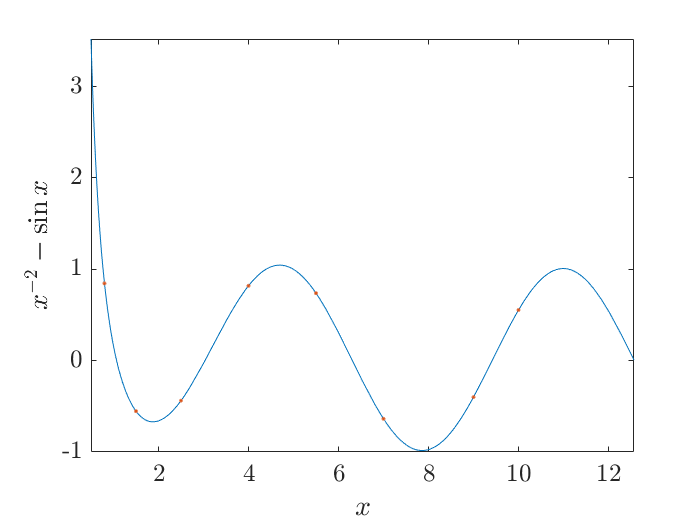
\includegraphics[scale=0.45]{graphics/plot-01.png}
    \caption{Plot of $f$ in $[1/2, 4 \pi]$}
  \end{figure}
  From the graph, it is clear that there are roots in the intervals
  $[0.8, 1.5], [2.5, 4], [5.5, 7]$ and $[9, 10]$.
  Using the secant method
  \lstinputlisting{scripts/algorithms/secant.m}
  the following code
  \lstinputlisting{scripts/problems/problem-01.m}
  outputs the approximated roots
  \verbatiminput{outputs/output-01.txt}
\end{solution}
